% lint-scope: appendix
\subsection{Further results}
\label{app:further}

\begin{figure}[tbp]
\centering
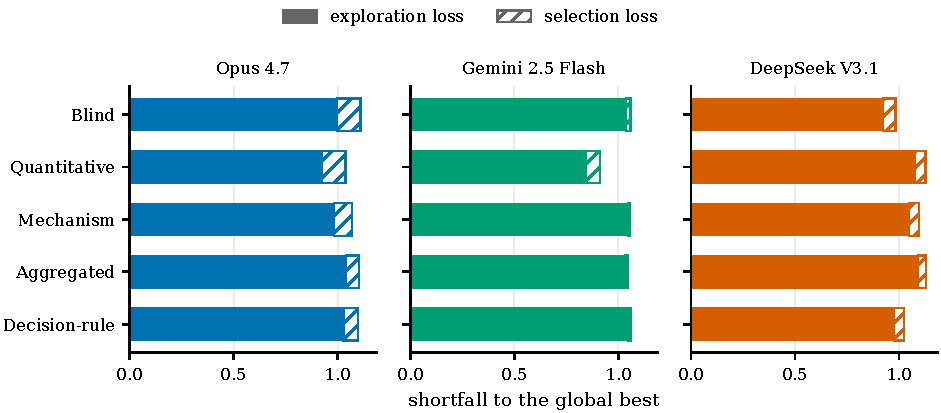
\includegraphics[width=\textwidth]{figA3_shortfall_global.pdf}
\caption{The shortfall to the global best in each cell, split into exploration loss and selection loss, which
sum to the whole. The guessing rule's own split, 0.67 to exploration and 0.23 to selection, is the reference point of
Figure~\ref{fig:loss}.}
\label{fig:shortfall_global}
\end{figure}

\paragraph{The scripted lab protocols.} Three scripted protocols spend the same 60 slots the way a wet lab
is often run, searching around their current best as the scripted rules do. Triplicate-everything measures 20 candidates three times,
66.7\% of slots on repeats. Duplicate-everything measures 30 twice, 50.0\%. Screen-then-confirm takes 48
single readings and then confirms the leaders, 20.0\%. These protocols are simulated, and a study with human
experimenters is future work.

\paragraph{Prompt conditions and exploration.} The explanatory conditions raise re-testing and cut
exploration. For Opus 4.7, distinct candidates fall from 11.34 under Blind to 9.02 under Mechanism and 6.99
under Aggregated, and its re-testing share rises from 75.4\% to 81.6\% and then 85.8\%. This is
descriptive across conditions and is not one of the pre-registered contrasts.

\paragraph{Final picks against the scripted rules.} Cell means of the final pick's true value run from
7.6308 to 7.8501. At $k^\ast$ the guessing rule reaches 7.8659 and the informed rule 7.9993. Against a
rule that never re-tests, the comparison depends on the reference. Five of the 15 cells sit above the guessing
rule's $k{=}0$ mean of 7.7098, two with intervals entirely above, and every cell sits below the informed
rule's 7.8862. The most exploratory cell reaches 39.2\% of the guessing rule's count of distinct candidates. Split
against the global best, exploration accounts for 0.8428 to 1.0928 of the shortfall and selection for 0.0087 to
0.1148, so in every cell exploration is 88.9\% to 99.2\% of the total and selection 0.8\% to 11.1\% (Figure~\ref{fig:shortfall_global}).

\paragraph{Rejections.} Cell means run 2.57 to 11.34 distinct candidates, against 28.94 for the guessing rule and
39.14 for the informed rule. Over all 5{,}075 prompt-study campaigns the agents were rejected 16.75 times per campaign and
lost 0.71 slots, against 83.02 and 11.70 for the guessing rule under the same rules. The agents were rejected less
often per campaign because they ordered far fewer new names: most of their slots went on re-tests. Per new name they
were rejected 72.2\% of the time, against 74.4\% for the guessing rule. New names are rejected orders plus
candidates measured, leaving out the starting candidate both are given. So the agents pick viable names about as
well as the guessing rule's neighbour sampling. Across the 15 cells the rate runs from 68.5\% to 89.0\%. Eight
of the 15 cells are rejected more often than the guessing rule and seven less often. The eight are Gemini 2.5
Flash in every condition except Quantitative, and DeepSeek V3.1 in every condition except Decision-rule.


\paragraph{The zero-noise run.} Here re-testing is counted after an agent's first repeat, as in
Figure~\ref{fig:zero}; the other zero-noise numbers in these appendices count all used slots. Re-testing after the first repeat at $\sigma=0$ runs from 51.8\% to 97.5\% across
the 15 cells, with a median of 90.6\%. The lowest cell is Quantitative with Opus 4.7, at 51.8\%, 95\%
interval [48.2\%, 55.4\%]. The highest is Aggregated with DeepSeek V3.1, at 97.5\%, [96.7\%, 98.3\%]. By
model, Opus 4.7 runs 51.8\% to 71.0\%, Gemini 2.5 Flash 76.8\% to 94.4\% and DeepSeek V3.1 94.1\% to
97.5\%. All 15 paired differences from the same cells with noise are negative, from $-35.0$ to $-0.9$ percentage
points, and 12 of 15 are significant at 0.05 after Holm correction within that run. Every cell pairs all 40 seeds. The size of the drop tracks the level a model starts from. Opus 4.7 falls furthest, and DeepSeek V3.1
falls least, from implied levels of 96.7\% to 98.5\%.

\subsection{The independent check}
\label{app:indep}

Each call shows one fixed round of an optimisation task. Every candidate is valid, so nothing is ever rejected. A
seven-round history is already measured, and the best candidate has already been measured twice. Three versions vary only what is true and what is said about measurement error: exact readings with exactness stated, exact
readings with nothing said, and noisy readings with the noise stated. Thirty paired histories per version, three
models, temperature 0, 270 calls. Scoring counts every proposal line the reply contains against four slots,
so a short reply is charged the shortfall, and a token outside the alphabet cannot count as a repeat.

\begin{table}[h]
\centering
\small
\caption{Share of the four chosen measurements that repeat an already-measured candidate.}
\begin{tabular}{lrrrr}
\toprule
model & exact, stated & exact, unstated & noisy, stated & noise effect (paired) \\
\midrule
Opus 4.7         & 24.2\% & 24.2\% & 61.7\% & $+37.5$ pp (SE 5.3) \\
Gemini 2.5 Flash & 45.0\% & 50.8\% & 95.0\% & $+50.0$ pp (SE 7.0) \\
DeepSeek V3.1    & 55.8\% & 49.2\% & 94.2\% & $+38.3$ pp (SE 8.3) \\
\bottomrule
\end{tabular}
\end{table}

A reading rule was fixed before any call. A repeat share of 25\% or more in the exact-stated version confirms
the behaviour; 5\% or less attributes it to our environment; anything between is partial.
Gemini 2.5 Flash and DeepSeek V3.1 clear the 25\% line. Opus 4.7 at 24.2\% falls just
below it, so two models give a clear reproduction and one is partial.

Stating that readings are exact made no detectable difference. The paired difference between saying
nothing and stating it is $+0.0$ pp (SE 2.4) for Opus 4.7, $+5.8$ (SE 7.1) for Gemini 2.5 Flash and $-6.7$
(SE 6.9) for DeepSeek V3.1. In the zero-noise run the noise effect looks small for Gemini 2.5 Flash and
DeepSeek V3.1 because their re-testing is already high with exact readings, at 81.6\% and 89.6\% of all
used slots against 51.4\% for Opus 4.7, each a mean over the five conditions.

\subsection{The prompt checks}
\label{app:prompt}

Three prompt changes were tested, each absent from the original prompts. The \emph{goal} option adds one sentence to the goal in the round and replacement prompts, the same in all five conditions: ``At the
end you will nominate one candidate, and your score is that candidate's true value.'' It says nothing about
readings, because the Blind condition withholds that readings carry error. The nomination prompt was left as it
was, since it already asks for the highest true score. The \emph{budget} option makes the replacement prompt's budget line
read ``15 rounds, 4 orders per round, 60 measurements in total.'' It had stated one order per round.

The \emph{free-rejection} option makes a rejected order free. In every prompt, the sentence on replacements and lost slots becomes
``An order for a non-viable candidate is rejected at no cost and you choose again. No slot is ever lost to a
non-viable order.'' The agent may then be asked again up to 20 times for one slot. A slot that reaches that cap
is lost and counted, and no slot in check B reached it. The guessing rule reached it in 353 of
its 1{,}500 campaigns at one re-test per round, and still lost 0.86 slots per campaign.

Check A used the goal and budget options and check B all three, each on Blind and Mechanism for all three models, on
the same 60 seeds. A rerun of the original prompts ran on the same day as check A. The registered statement for check B reads ``rejection risk does not produce the habit''. Intervals are 95\% percentile bootstraps over the paired
campaigns. In check B the final pick of Opus 4.7 under Mechanism fell by 0.1340 [$-0.2324$, $-0.0347$].


\section{Three exploratory experiments}
\label{app:panels}


\paragraph{Temperature.} Three models under Mechanism at temperature 1.0, on the grid's own seeds. Re-testing moves by $-0.3$
percentage points (SE 0.8) for Opus 4.7 and $-1.0$ (SE 0.3) for DeepSeek V3.1, and falls
5.5 (SE 1.0) for Gemini 2.5 Flash, which leaves it at 89.9\% of slots. The final pick
moves by at most 0.07 in either direction, with standard errors of 0.04 to 0.06.

\paragraph{Reasoning.}
\label{app:reasoning}
This experiment runs two of the five conditions on two of the three models, at reasoning effort
medium, paired by seed against the prompt study with 35 to 40 seeds per cell after exclusions. Holm correction runs across
its four cells only.

Reasoning shifted agents from re-testing toward exploration and their picks worsened, mainly because they
found worse candidates. The re-testing share falls by 7.5 to 12.4 percentage points and distinct candidates
rise by 3.7 to 7.1 per campaign in all four cells. The final pick's true value falls by 0.099 to 0.263,
and all four cells reject at 0.05 after Holm. The true value of the best candidate the agent measured drops
from 7.6854--7.7387 in the prompt study to 7.5302--7.6253 under reasoning, so exploration loss rises by $+0.06$ to $+0.19$, and selection loss by only $+0.007$ to $+0.085$. Keeping the nine excluded campaigns
leaves the comparison unchanged: with all 40 paired seeds the differences are $-0.0987$, $-0.2528$,
$-0.2016$ and $-0.2338$, and all four still reject.

In 9 of 80 Gemini 2.5 Flash reasoning campaigns the model returned no final answer, eight of them at the 6{,}000-token
output limit. These are excluded, and the check above includes them.

\paragraph{Biology framing.}
\label{app:bio}
Three cells of 40 campaigns on three models, all under the Blind condition, differing in one sentence
of the prompt and in $\sigma$. The added sentence gives the agent a wet-lab role, so the result covers only what one sentence of lab
context does to the behaviour. The candidates are four letters from A to T. Seventeen of the twenty letters are amino-acid codes. The landscape is generated, so a biochemical intuition the framing evokes has nothing to attach to.

The role lowers re-testing in all three models against the same prompt without it: $-6.5$ percentage points
for Opus 4.7 $[-8.5, -4.5]$, $-9.8$ for Gemini 2.5 Flash $[-12.7, -7.0]$ and $-2.9$ for
DeepSeek V3.1 $[-4.7, -1.2]$. Re-testing persists under the role with exact readings, at 49.1\% to
86.4\% of slots. The same persistence appears with no role at all: the zero-noise run's own Blind cells, which carry the
prompt these role cells are built on, sit at 52.6\%, 92.9\% and 88.0\% of all used slots. Within this experiment, exact readings lower re-testing against the role cell by 19.8, 8.3 and 1.8 percentage points, paired by
seed, with DeepSeek V3.1's interval including zero.

\section{A pre-registered replication of the Decision-rule result}
\label{app:replication}

One confirmatory contrast survived Holm correction: DeepSeek V3.1's final picks were better under
Decision-rule than under Mechanism. We ran that comparison again on 120 seeds that no earlier run had used.
The design, the outcome and the reading rule were fixed before any call. The landscape, the prompts and
the settings were those of the prompt study.

The outcome is the paired difference in the final pick's true value, Decision-rule minus Mechanism. One
Decision-rule campaign whose nomination did not parse is excluded, as in the prompt study's analysis, which leaves 119
pairs. The rule, fixed in advance, has three readings. A positive mean whose 95\% bootstrap interval excludes
zero replicates. A positive mean whose interval includes zero reads as ``direction holds, not significant''.
A mean at or below zero does not replicate.

The mean difference is $+0.008$, with a 95\% bootstrap interval of $[-0.036, +0.052]$. By the rule, the
direction holds and the difference is not significant. Of the 119 pairs, 37 improved, 33 got worse and 49
were unchanged. The interval's upper end lies below the original estimate of $+0.0699$ and below 0.06, the smallest
effect the study was designed to detect.

Not pre-registered: because the landscape and settings are the same, the replication's conditions can be set against the original run's. The Decision-rule means match: 7.736 originally and 7.736 in the replication. The
Mechanism mean rose from 7.664 to 7.728, a difference of $+0.064$ (SE 0.023). This is consistent with the
original gap coming mostly from a Mechanism sample that happened to score low.

\section{The learnability simulation}
\label{app:sim}

This simulation makes no model calls. It runs the informed and the guessing rule at $K \in \{1,2,3\}$ and at
noise of 0.5, 1 and 2 times ours, 18 settings in all. Each uses 200 fresh landscapes, one per seed, and training and
held-out landscapes come from separate seed ranges.

Trained on the environment's reward alone, a two-parameter learner that chooses the number of re-tests and the
selection rule settles on $k=1$ with the registered selection rule of Section~\ref{sec:under}. That is $k^\ast$ or tied with $k^\ast$ in all 18
simulated settings. Sweeping $k$ gives $k^\ast = 1$ in 13 settings, $k^\ast = 2$ in 3 and $k^\ast = 0$ in 2. In 16 of the 18 the
gap between $k^\ast$ and its runner-up sits inside two standard errors, so most settings are ties. Raw paired
differences between the policy at $k^\ast$ with the registered selection rule and the rule that never re-tests run $-0.0077$ to $+0.2231$
on the held-out landscapes, and both negative values are at half noise.

\begin{figure}[tbp]
\centering
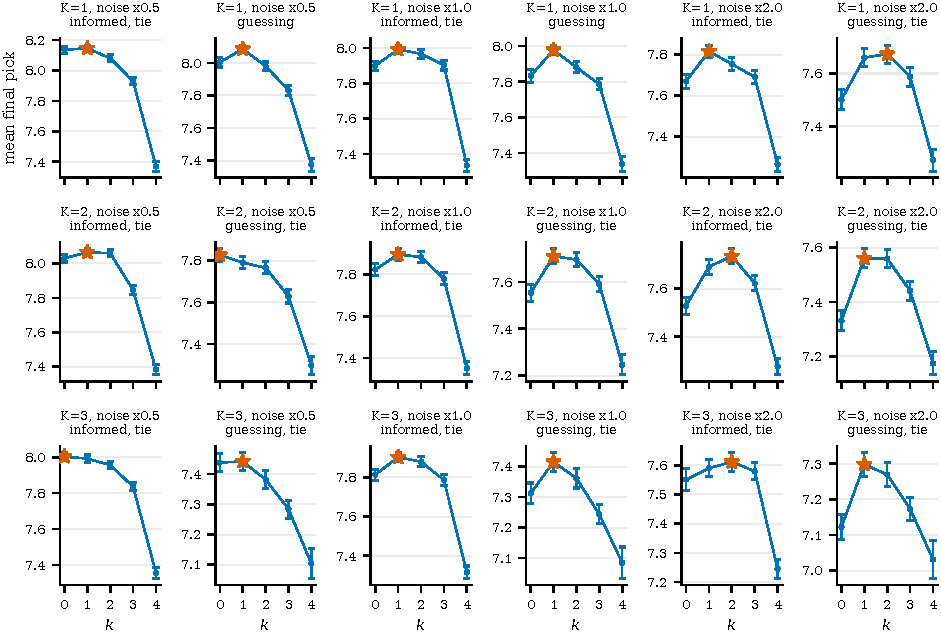
\includegraphics[width=\textwidth]{figA2_simulation.pdf}
\caption{The learnability simulation: mean final pick against $k$, the slots per round spent re-testing
the current best, one panel per setting of ruggedness $K$, noise and rule, over 200 generated landscapes per
setting, with standard errors. The star marks the best $k$. A panel marked \emph{tie} is one where the paired gap
to the runner-up is inside two of its own standard errors.}
\label{fig:sim}
\end{figure}

The right rate depends on the noise. It is zero when readings are exact. In the simulation one repeat per round is best
or tied in all 18 settings. At half noise, never re-testing ties with one repeat in two settings at 200
landscapes, and at 1{,}500 landscapes the best is never zero. 

\paragraph{The normalised score and collapses.} The pre-registered score rescales each result between those of
two scripted endpoints. Across landscapes those endpoints move by more than the gap between them, so a held-out score
rescaled with training endpoints is unstable: 0.122 to 7.765 across the 16 cells where it is defined.
Rescored with endpoints from the same held-out landscapes it runs 0.784 to 1.000. It is exactly 1.000 in the 11 cells
where $k^\ast = 1$ and the score is defined, because the learner selects that policy, and undefined in four cells at
half noise, where the held-out span is zero or negative. No claim in this paper depends on it. The guessing rule's
means at high re-testing are over surviving campaigns, since a campaign collapses when fewer than two candidates are
measured: at $K=3$, 138 of 200 campaigns collapse at $k=4$ and 12 of 200 at $k=3$.

\paragraph{The larger run.} At 1{,}500 landscapes per setting the picture holds: one
re-test a round is best or tied in all 18 settings. The three settings where two came out ahead
are all at double noise and all within two standard errors. Rescored with held-out endpoints, the learner
selects one re-test a round with the registered selection rule in every setting. It scores exactly 1.000 in the 15 settings where
$k^\ast = 1$ and between 0.819 and 0.925 in the other three. Figure~\ref{fig:sim} is drawn at 200 landscapes,
the pre-registered primary, since only that run recorded a standard error for each $k$.
